\documentclass[tikz,border=3pt]{standalone}
\usepackage[utf8]{inputenc}
\usepackage[T1]{fontenc}
\usepackage{lmodern}
\renewcommand{\familydefault}{\sfdefault}
\usepackage{sansmath}\sansmath
\usepackage{chemfig}
\usepackage{pgfplots}\pgfplotsset{compat=1.18,/pgf/number format/use comma,/pgf/number format/1000 sep={.}}
\usetikzlibrary{arrows.meta,calc,positioning,decorations.pathmorphing,patterns}
% paleta del sitio
\definecolor{nar}{HTML}{E8680C}\definecolor{narc}{HTML}{FFB35C}\definecolor{hielo}{HTML}{FFF3E8}
\definecolor{tinta}{HTML}{1D1D1F}\definecolor{gris}{HTML}{6E6E73}\definecolor{lila}{HTML}{7C5CF0}
\definecolor{azul}{HTML}{2F6FD6}\definecolor{menta}{HTML}{17A673}\definecolor{coral}{HTML}{E8342A}
\begin{document}
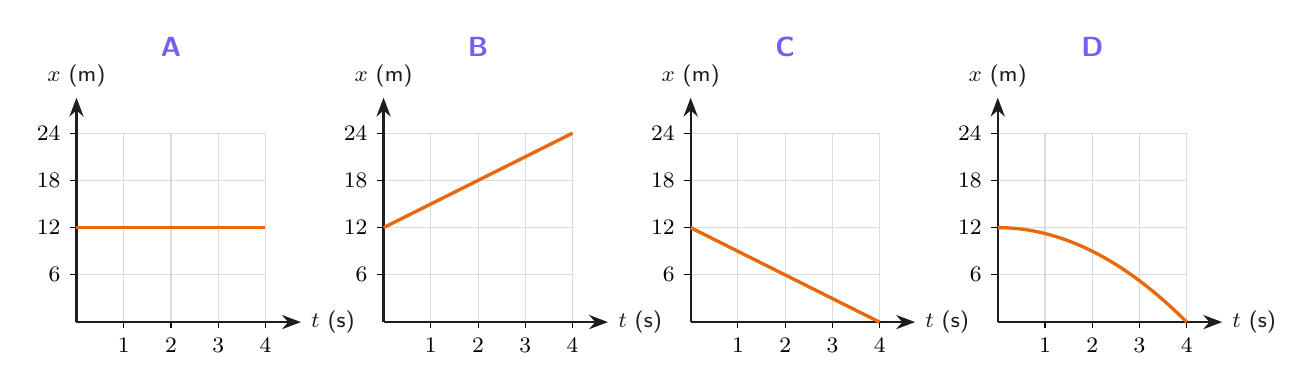
\begin{tikzpicture}[font=\footnotesize,>={Stealth[length=2.4mm]},]
\begin{scope}[shift={(0.0,0)}]
\foreach \y in {0.6,1.2,1.8,2.4} \draw[gris!25] (0,\y) -- (2.4,\y);
\foreach \x in {0.6,1.2,1.8,2.4} \draw[gris!25] (\x,0) -- (\x,2.4);
\draw[->,thick,tinta] (0,0) -- (2.85,0) node[right] {$t$ (s)};
\draw[->,thick,tinta] (0,0) -- (0,2.85) node[above] {$x$ (m)};
\foreach \x/\l in {0.6/1,1.2/2,1.8/3,2.4/4} \draw (\x,0) -- ++(0,-0.08) node[below] {$\l$};
\foreach \y/\l in {0.6/6,1.2/12,1.8/18,2.4/24} \draw (0,\y) -- ++(-0.08,0) node[left] {$\l$};
\draw[very thick,nar] (0,1.2) -- (2.4,1.2);
\node[font=\normalsize\bfseries,text=lila] at (1.2,3.5) {A};
\end{scope}
\begin{scope}[shift={(3.9,0)}]
\foreach \y in {0.6,1.2,1.8,2.4} \draw[gris!25] (0,\y) -- (2.4,\y);
\foreach \x in {0.6,1.2,1.8,2.4} \draw[gris!25] (\x,0) -- (\x,2.4);
\draw[->,thick,tinta] (0,0) -- (2.85,0) node[right] {$t$ (s)};
\draw[->,thick,tinta] (0,0) -- (0,2.85) node[above] {$x$ (m)};
\foreach \x/\l in {0.6/1,1.2/2,1.8/3,2.4/4} \draw (\x,0) -- ++(0,-0.08) node[below] {$\l$};
\foreach \y/\l in {0.6/6,1.2/12,1.8/18,2.4/24} \draw (0,\y) -- ++(-0.08,0) node[left] {$\l$};
\draw[very thick,nar] (0,1.2) -- (2.4,2.4);
\node[font=\normalsize\bfseries,text=lila] at (1.2,3.5) {B};
\end{scope}
\begin{scope}[shift={(7.8,0)}]
\foreach \y in {0.6,1.2,1.8,2.4} \draw[gris!25] (0,\y) -- (2.4,\y);
\foreach \x in {0.6,1.2,1.8,2.4} \draw[gris!25] (\x,0) -- (\x,2.4);
\draw[->,thick,tinta] (0,0) -- (2.85,0) node[right] {$t$ (s)};
\draw[->,thick,tinta] (0,0) -- (0,2.85) node[above] {$x$ (m)};
\foreach \x/\l in {0.6/1,1.2/2,1.8/3,2.4/4} \draw (\x,0) -- ++(0,-0.08) node[below] {$\l$};
\foreach \y/\l in {0.6/6,1.2/12,1.8/18,2.4/24} \draw (0,\y) -- ++(-0.08,0) node[left] {$\l$};
\draw[very thick,nar] (0,1.2) -- (2.4,0);
\node[font=\normalsize\bfseries,text=lila] at (1.2,3.5) {C};
\end{scope}
\begin{scope}[shift={(11.7,0)}]
\foreach \y in {0.6,1.2,1.8,2.4} \draw[gris!25] (0,\y) -- (2.4,\y);
\foreach \x in {0.6,1.2,1.8,2.4} \draw[gris!25] (\x,0) -- (\x,2.4);
\draw[->,thick,tinta] (0,0) -- (2.85,0) node[right] {$t$ (s)};
\draw[->,thick,tinta] (0,0) -- (0,2.85) node[above] {$x$ (m)};
\foreach \x/\l in {0.6/1,1.2/2,1.8/3,2.4/4} \draw (\x,0) -- ++(0,-0.08) node[below] {$\l$};
\foreach \y/\l in {0.6/6,1.2/12,1.8/18,2.4/24} \draw (0,\y) -- ++(-0.08,0) node[left] {$\l$};
\draw[very thick,nar,domain=0:2.4,smooth,variable=\t] plot (\t,{1.2-1.2*(\t/2.4)^2});
\node[font=\normalsize\bfseries,text=lila] at (1.2,3.5) {D};
\end{scope}
\end{tikzpicture}
\end{document}
